\documentclass[]{article}
\usepackage{lmodern}
\usepackage{amssymb,amsmath}
\usepackage{ifxetex,ifluatex}
\usepackage{fixltx2e} % provides \textsubscript
\ifnum 0\ifxetex 1\fi\ifluatex 1\fi=0 % if pdftex
  \usepackage[T1]{fontenc}
  \usepackage[utf8]{inputenc}
\else % if luatex or xelatex
  \ifxetex
    \usepackage{mathspec}
  \else
    \usepackage{fontspec}
  \fi
  \defaultfontfeatures{Ligatures=TeX,Scale=MatchLowercase}
\fi
% use upquote if available, for straight quotes in verbatim environments
\IfFileExists{upquote.sty}{\usepackage{upquote}}{}
% use microtype if available
\IfFileExists{microtype.sty}{%
\usepackage{microtype}
\UseMicrotypeSet[protrusion]{basicmath} % disable protrusion for tt fonts
}{}
\usepackage[margin=1in]{geometry}
\usepackage{hyperref}
\hypersetup{unicode=true,
            pdftitle={Reproducible Research: Peer Assessment 1},
            pdfborder={0 0 0},
            breaklinks=true}
\urlstyle{same}  % don't use monospace font for urls
\usepackage{color}
\usepackage{fancyvrb}
\newcommand{\VerbBar}{|}
\newcommand{\VERB}{\Verb[commandchars=\\\{\}]}
\DefineVerbatimEnvironment{Highlighting}{Verbatim}{commandchars=\\\{\}}
% Add ',fontsize=\small' for more characters per line
\usepackage{framed}
\definecolor{shadecolor}{RGB}{248,248,248}
\newenvironment{Shaded}{\begin{snugshade}}{\end{snugshade}}
\newcommand{\KeywordTok}[1]{\textcolor[rgb]{0.13,0.29,0.53}{\textbf{#1}}}
\newcommand{\DataTypeTok}[1]{\textcolor[rgb]{0.13,0.29,0.53}{#1}}
\newcommand{\DecValTok}[1]{\textcolor[rgb]{0.00,0.00,0.81}{#1}}
\newcommand{\BaseNTok}[1]{\textcolor[rgb]{0.00,0.00,0.81}{#1}}
\newcommand{\FloatTok}[1]{\textcolor[rgb]{0.00,0.00,0.81}{#1}}
\newcommand{\ConstantTok}[1]{\textcolor[rgb]{0.00,0.00,0.00}{#1}}
\newcommand{\CharTok}[1]{\textcolor[rgb]{0.31,0.60,0.02}{#1}}
\newcommand{\SpecialCharTok}[1]{\textcolor[rgb]{0.00,0.00,0.00}{#1}}
\newcommand{\StringTok}[1]{\textcolor[rgb]{0.31,0.60,0.02}{#1}}
\newcommand{\VerbatimStringTok}[1]{\textcolor[rgb]{0.31,0.60,0.02}{#1}}
\newcommand{\SpecialStringTok}[1]{\textcolor[rgb]{0.31,0.60,0.02}{#1}}
\newcommand{\ImportTok}[1]{#1}
\newcommand{\CommentTok}[1]{\textcolor[rgb]{0.56,0.35,0.01}{\textit{#1}}}
\newcommand{\DocumentationTok}[1]{\textcolor[rgb]{0.56,0.35,0.01}{\textbf{\textit{#1}}}}
\newcommand{\AnnotationTok}[1]{\textcolor[rgb]{0.56,0.35,0.01}{\textbf{\textit{#1}}}}
\newcommand{\CommentVarTok}[1]{\textcolor[rgb]{0.56,0.35,0.01}{\textbf{\textit{#1}}}}
\newcommand{\OtherTok}[1]{\textcolor[rgb]{0.56,0.35,0.01}{#1}}
\newcommand{\FunctionTok}[1]{\textcolor[rgb]{0.00,0.00,0.00}{#1}}
\newcommand{\VariableTok}[1]{\textcolor[rgb]{0.00,0.00,0.00}{#1}}
\newcommand{\ControlFlowTok}[1]{\textcolor[rgb]{0.13,0.29,0.53}{\textbf{#1}}}
\newcommand{\OperatorTok}[1]{\textcolor[rgb]{0.81,0.36,0.00}{\textbf{#1}}}
\newcommand{\BuiltInTok}[1]{#1}
\newcommand{\ExtensionTok}[1]{#1}
\newcommand{\PreprocessorTok}[1]{\textcolor[rgb]{0.56,0.35,0.01}{\textit{#1}}}
\newcommand{\AttributeTok}[1]{\textcolor[rgb]{0.77,0.63,0.00}{#1}}
\newcommand{\RegionMarkerTok}[1]{#1}
\newcommand{\InformationTok}[1]{\textcolor[rgb]{0.56,0.35,0.01}{\textbf{\textit{#1}}}}
\newcommand{\WarningTok}[1]{\textcolor[rgb]{0.56,0.35,0.01}{\textbf{\textit{#1}}}}
\newcommand{\AlertTok}[1]{\textcolor[rgb]{0.94,0.16,0.16}{#1}}
\newcommand{\ErrorTok}[1]{\textcolor[rgb]{0.64,0.00,0.00}{\textbf{#1}}}
\newcommand{\NormalTok}[1]{#1}
\usepackage{graphicx,grffile}
\makeatletter
\def\maxwidth{\ifdim\Gin@nat@width>\linewidth\linewidth\else\Gin@nat@width\fi}
\def\maxheight{\ifdim\Gin@nat@height>\textheight\textheight\else\Gin@nat@height\fi}
\makeatother
% Scale images if necessary, so that they will not overflow the page
% margins by default, and it is still possible to overwrite the defaults
% using explicit options in \includegraphics[width, height, ...]{}
\setkeys{Gin}{width=\maxwidth,height=\maxheight,keepaspectratio}
\IfFileExists{parskip.sty}{%
\usepackage{parskip}
}{% else
\setlength{\parindent}{0pt}
\setlength{\parskip}{6pt plus 2pt minus 1pt}
}
\setlength{\emergencystretch}{3em}  % prevent overfull lines
\providecommand{\tightlist}{%
  \setlength{\itemsep}{0pt}\setlength{\parskip}{0pt}}
\setcounter{secnumdepth}{0}
% Redefines (sub)paragraphs to behave more like sections
\ifx\paragraph\undefined\else
\let\oldparagraph\paragraph
\renewcommand{\paragraph}[1]{\oldparagraph{#1}\mbox{}}
\fi
\ifx\subparagraph\undefined\else
\let\oldsubparagraph\subparagraph
\renewcommand{\subparagraph}[1]{\oldsubparagraph{#1}\mbox{}}
\fi

%%% Use protect on footnotes to avoid problems with footnotes in titles
\let\rmarkdownfootnote\footnote%
\def\footnote{\protect\rmarkdownfootnote}

%%% Change title format to be more compact
\usepackage{titling}

% Create subtitle command for use in maketitle
\newcommand{\subtitle}[1]{
  \posttitle{
    \begin{center}\large#1\end{center}
    }
}

\setlength{\droptitle}{-2em}
  \title{Reproducible Research: Peer Assessment 1}
  \pretitle{\vspace{\droptitle}\centering\huge}
  \posttitle{\par}
  \author{}
  \preauthor{}\postauthor{}
  \date{}
  \predate{}\postdate{}


\begin{document}
\maketitle

\subsection{Loading and preprocessing the
data}\label{loading-and-preprocessing-the-data}

\begin{Shaded}
\begin{Highlighting}[]
\KeywordTok{setwd}\NormalTok{(}\StringTok{"~/DataScience/R_Research/RepData_PeerAssessment1"}\NormalTok{)}
\KeywordTok{unzip}\NormalTok{(}\StringTok{"activity.zip"}\NormalTok{, }\DataTypeTok{exdir =} \KeywordTok{getwd}\NormalTok{())}
\NormalTok{Activity_Data <-}\StringTok{ }\KeywordTok{read.csv}\NormalTok{(}\StringTok{"C:/Users/Caremecc/Documents/DataScience/R_Research/RepData_PeerAssessment1/activity.csv"}\NormalTok{, }\DataTypeTok{header =} \OtherTok{TRUE}\NormalTok{)}
\end{Highlighting}
\end{Shaded}

\subsection{What is mean total number of steps taken per
day?}\label{what-is-mean-total-number-of-steps-taken-per-day}

\subsubsection{1. Total number of steps taken per
day.}\label{total-number-of-steps-taken-per-day.}

\begin{Shaded}
\begin{Highlighting}[]
\NormalTok{tSteps <-}\StringTok{ }\KeywordTok{sum}\NormalTok{(Activity_Data}\OperatorTok{$}\NormalTok{steps, }\DataTypeTok{na.rm =} \OtherTok{TRUE}\NormalTok{)}
\NormalTok{tSteps}
\end{Highlighting}
\end{Shaded}

\begin{verbatim}
## [1] 570608
\end{verbatim}

\subsubsection{2. Histogram of the total number of steps taken each
day.}\label{histogram-of-the-total-number-of-steps-taken-each-day.}

\begin{Shaded}
\begin{Highlighting}[]
\NormalTok{##calculating and storing the total number of steps in to the variable "tSteps"}
\NormalTok{tSteps <-}\StringTok{ }\KeywordTok{aggregate}\NormalTok{(steps }\OperatorTok{~}\StringTok{ }\NormalTok{date, }\DataTypeTok{data =}\NormalTok{ Activity_Data, }\DataTypeTok{FUN =}\NormalTok{ sum, }\DataTypeTok{na.rm =} \OtherTok{TRUE}\NormalTok{)}

\NormalTok{##Generate the histogram of the total number of steps taken each day.}
\KeywordTok{hist}\NormalTok{(tSteps}\OperatorTok{$}\NormalTok{step, }\DataTypeTok{xlab =} \StringTok{"Number of Steps"}\NormalTok{, }\DataTypeTok{main =} \StringTok{"Number of Steps taken per day"}\NormalTok{, }\DataTypeTok{col =} \StringTok{"green"}\NormalTok{)}
\end{Highlighting}
\end{Shaded}

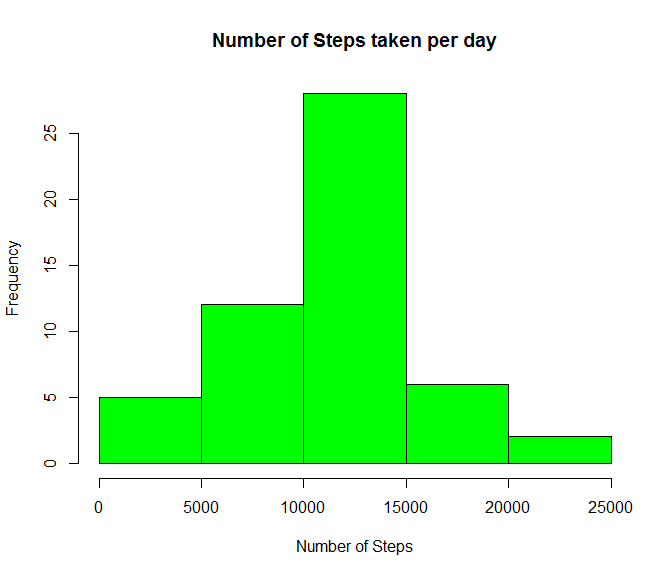
\includegraphics{PA1_template_files/figure-latex/Plot_1-1.pdf}

\subsubsection{3. Calculate and report the mean and median of the total
number of steps taken per
day}\label{calculate-and-report-the-mean-and-median-of-the-total-number-of-steps-taken-per-day}

\begin{Shaded}
\begin{Highlighting}[]
\NormalTok{##Mean number of steps}
\NormalTok{tSteps_mean <-}\StringTok{ }\KeywordTok{mean}\NormalTok{(tSteps}\OperatorTok{$}\NormalTok{steps)}

\NormalTok{##Mean number of steps}
\NormalTok{tSteps_median <-}\StringTok{ }\KeywordTok{median}\NormalTok{(tSteps}\OperatorTok{$}\NormalTok{steps)}

\NormalTok{tSteps_mean}
\end{Highlighting}
\end{Shaded}

\begin{verbatim}
## [1] 10766.19
\end{verbatim}

\begin{Shaded}
\begin{Highlighting}[]
\NormalTok{tSteps_median}
\end{Highlighting}
\end{Shaded}

\begin{verbatim}
## [1] 10765
\end{verbatim}

\subsection{What is the average daily activity
pattern?}\label{what-is-the-average-daily-activity-pattern}

\subsubsection{\texorpdfstring{1. Time series plot (i.e.~type = ``1'')
of the 5-minute interval (x-axis) and the average number of steps taken,
averaged across all days
(y-axis)}{1. Time series plot (i.e.~type = 1) of the 5-minute interval (x-axis) and the average number of steps taken, averaged across all days (y-axis)}}\label{time-series-plot-i.e.type-1-of-the-5-minute-interval-x-axis-and-the-average-number-of-steps-taken-averaged-across-all-days-y-axis}

\begin{Shaded}
\begin{Highlighting}[]
\KeywordTok{library}\NormalTok{(ggplot2)}
\NormalTok{five_min_interval <-}\StringTok{ }\KeywordTok{aggregate}\NormalTok{(steps }\OperatorTok{~}\StringTok{ }\NormalTok{interval, }\DataTypeTok{data =}\NormalTok{ Activity_Data, }\DataTypeTok{FUN =}\NormalTok{ mean, }\DataTypeTok{na.rm =} \OtherTok{TRUE}\NormalTok{)}
\KeywordTok{ggplot}\NormalTok{(}\DataTypeTok{data =}\NormalTok{ five_min_interval, }\KeywordTok{aes}\NormalTok{(}\DataTypeTok{x =}\NormalTok{ interval, }\DataTypeTok{y =}\NormalTok{ steps)) }\OperatorTok{+}
\StringTok{  }\KeywordTok{geom_line}\NormalTok{() }\OperatorTok{+}\StringTok{ }
\StringTok{  }\KeywordTok{ggtitle}\NormalTok{(}\StringTok{"The average daily activity pattern"}\NormalTok{) }\OperatorTok{+}
\StringTok{  }\KeywordTok{xlab}\NormalTok{(}\StringTok{"5-minute interval"}\NormalTok{) }\OperatorTok{+}
\StringTok{  }\KeywordTok{ylab}\NormalTok{(}\StringTok{"Average number of steps taken"}\NormalTok{)}
\end{Highlighting}
\end{Shaded}

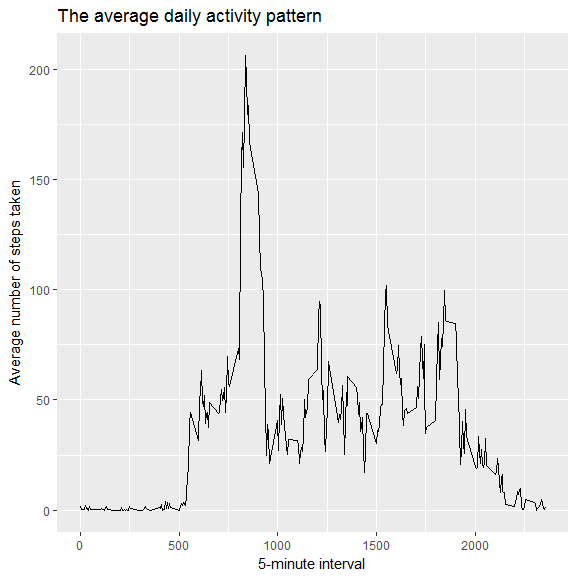
\includegraphics{PA1_template_files/figure-latex/Plot_2-1.pdf}

\begin{Shaded}
\begin{Highlighting}[]
\NormalTok{MaxSteps <-}\StringTok{ }\NormalTok{five_min_interval[}\KeywordTok{which.max}\NormalTok{(five_min_interval}\OperatorTok{$}\NormalTok{steps),]}

\NormalTok{MaxSteps}
\end{Highlighting}
\end{Shaded}

\begin{verbatim}
##     interval    steps
## 104      835 206.1698
\end{verbatim}

\subsection{Imputing missing values}\label{imputing-missing-values}

\subsubsection{1. Calculate and report the total number of missing
values in the
dataset}\label{calculate-and-report-the-total-number-of-missing-values-in-the-dataset}

\begin{Shaded}
\begin{Highlighting}[]
\NormalTok{total_NA <-}\StringTok{ }\KeywordTok{sum}\NormalTok{(}\KeywordTok{is.na}\NormalTok{(Activity_Data}\OperatorTok{$}\NormalTok{steps))}

\NormalTok{total_NA}
\end{Highlighting}
\end{Shaded}

\begin{verbatim}
## [1] 2304
\end{verbatim}

\subsubsection{2. Strategy for filling in all of the missing values in
the
dataset.}\label{strategy-for-filling-in-all-of-the-missing-values-in-the-dataset.}

The missing value will be imputted into the dataset using the 5 day
average of the respective 5 minute interval.

\subsubsection{3. Create a new dataset that is equal to the original
dataset but with the missing values filled
in.}\label{create-a-new-dataset-that-is-equal-to-the-original-dataset-but-with-the-missing-values-filled-in.}

\subsubsection{Imputting the missing values in to the
dataset.}\label{imputting-the-missing-values-in-to-the-dataset.}

\begin{Shaded}
\begin{Highlighting}[]
\NormalTok{imputted_act_Data <-}\StringTok{ }\KeywordTok{transform}\NormalTok{(Activity_Data, }\DataTypeTok{steps =} \KeywordTok{ifelse}\NormalTok{(}\KeywordTok{is.na}\NormalTok{(Activity_Data}\OperatorTok{$}\NormalTok{steps), five_min_interval}\OperatorTok{$}\NormalTok{steps[}\KeywordTok{match}\NormalTok{(Activity_Data}\OperatorTok{$}\NormalTok{interval, five_min_interval}\OperatorTok{$}\NormalTok{interval)],}
\NormalTok{                                                             Activity_Data}\OperatorTok{$}\NormalTok{steps))}
\end{Highlighting}
\end{Shaded}

\subsubsection{4. Make a histogram of the total number of steps taken
each day and calculate and report the mean and median total number of
steps taken per
day.}\label{make-a-histogram-of-the-total-number-of-steps-taken-each-day-and-calculate-and-report-the-mean-and-median-total-number-of-steps-taken-per-day.}

\begin{Shaded}
\begin{Highlighting}[]
\NormalTok{New_tSteps <-}\StringTok{ }\KeywordTok{aggregate}\NormalTok{(steps }\OperatorTok{~}\StringTok{ }\NormalTok{date, }\DataTypeTok{data =}\NormalTok{ imputted_act_Data, }\DataTypeTok{FUN =}\NormalTok{ sum, }\DataTypeTok{na.rm =} \OtherTok{TRUE}\NormalTok{)}

\CommentTok{#Histogram}
\KeywordTok{hist}\NormalTok{(New_tSteps}\OperatorTok{$}\NormalTok{steps, }\DataTypeTok{xlab =} \StringTok{"Number of Steps"}\NormalTok{, }\DataTypeTok{main =} \StringTok{"Number of Steps taken per day"}\NormalTok{, }\DataTypeTok{col =} \StringTok{"green"}\NormalTok{)}
\end{Highlighting}
\end{Shaded}

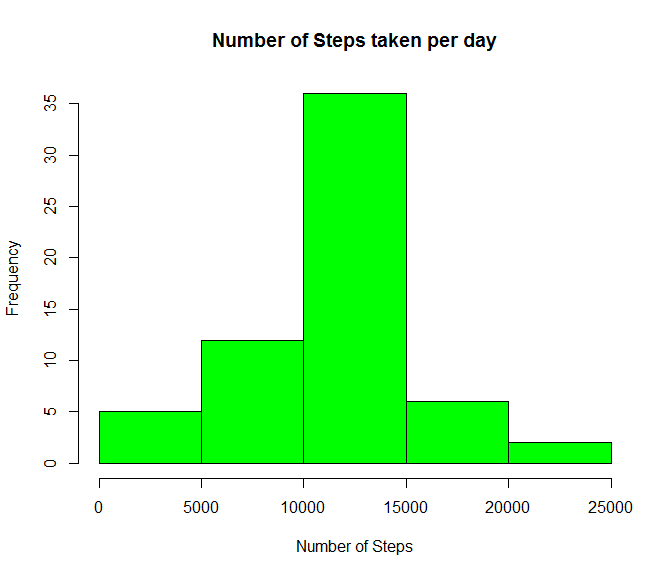
\includegraphics{PA1_template_files/figure-latex/Plot_3-1.pdf}

\subsubsection{The values does look different in comparison to the
estimates derived from the first set of data without the imputation.See
results
below.}\label{the-values-does-look-different-in-comparison-to-the-estimates-derived-from-the-first-set-of-data-without-the-imputation.see-results-below.}

\begin{Shaded}
\begin{Highlighting}[]
\CommentTok{#Mean number of steps}
\NormalTok{NewtSteps_mean <-}\StringTok{ }\KeywordTok{mean}\NormalTok{(New_tSteps}\OperatorTok{$}\NormalTok{steps)}

\CommentTok{#Mean number of steps}
\NormalTok{NewtSteps_median <-}\StringTok{ }\KeywordTok{median}\NormalTok{(New_tSteps}\OperatorTok{$}\NormalTok{steps)}

\NormalTok{NewtSteps_mean}
\end{Highlighting}
\end{Shaded}

\begin{verbatim}
## [1] 10766.19
\end{verbatim}

\begin{Shaded}
\begin{Highlighting}[]
\NormalTok{NewtSteps_median}
\end{Highlighting}
\end{Shaded}

\begin{verbatim}
## [1] 10766.19
\end{verbatim}

\subsubsection{The impact of the imputed values shows that the gap
between the mean and median have close, they are both the same
figure.}\label{the-impact-of-the-imputed-values-shows-that-the-gap-between-the-mean-and-median-have-close-they-are-both-the-same-figure.}

\subsection{Are there differences in activity patterns between weekdays
and
weekends?}\label{are-there-differences-in-activity-patterns-between-weekdays-and-weekends}

\subsubsection{\texorpdfstring{1. Create the factor variable in the
datasetwithtwo levels - ``weekday'' and ``weekdend'' indicating whether
a given date is a weekday or weekend
day.}{1. Create the factor variable in the datasetwithtwo levels - weekday and weekdend indicating whether a given date is a weekday or weekend day.}}\label{create-the-factor-variable-in-the-datasetwithtwo-levels---weekday-and-weekdend-indicating-whether-a-given-date-is-a-weekday-or-weekend-day.}

\begin{Shaded}
\begin{Highlighting}[]
\NormalTok{wday_end <-}\StringTok{ }\ControlFlowTok{function}\NormalTok{(date) \{}
\NormalTok{  day <-}\StringTok{ }\KeywordTok{weekdays}\NormalTok{(date)}
  \ControlFlowTok{if}\NormalTok{ (day }\OperatorTok\StringTok{ }\KeywordTok{c}\NormalTok{(}\StringTok{"Monday"}\NormalTok{, }\StringTok{"Tuesday"}\NormalTok{, }\StringTok{"Wednesday"}\NormalTok{, }\StringTok{"Thursday"}\NormalTok{, }\StringTok{"Friday"}\NormalTok{))}
    \KeywordTok{return}\NormalTok{(}\StringTok{"weekday"}\NormalTok{) }\ControlFlowTok{else} \ControlFlowTok{if}\NormalTok{ (day }\OperatorTok\StringTok{ }\KeywordTok{c}\NormalTok{(}\StringTok{"Saturday"}\NormalTok{, }\StringTok{"Sunday"}\NormalTok{))}
      \KeywordTok{return}\NormalTok{(}\StringTok{"weekend"}\NormalTok{) }\ControlFlowTok{else} \KeywordTok{stop}\NormalTok{(}\StringTok{"Invalid Date"}\NormalTok{)}
\NormalTok{\}}

\NormalTok{imputted_act_Data}\OperatorTok{$}\NormalTok{date <-}\StringTok{ }\KeywordTok{as.Date}\NormalTok{(imputted_act_Data}\OperatorTok{$}\NormalTok{date)}
\NormalTok{imputted_act_Data}\OperatorTok{$}\NormalTok{day <-}\StringTok{ }\KeywordTok{sapply}\NormalTok{(imputted_act_Data}\OperatorTok{$}\NormalTok{date, }\DataTypeTok{FUN =}\NormalTok{ wday_end)}
\end{Highlighting}
\end{Shaded}

\subsubsection{2. Make a panel plot containing a time series plot of the
5 minute interval and the average number of steps taken, averaged across
all weekday days and weekend
days.}\label{make-a-panel-plot-containing-a-time-series-plot-of-the-5-minute-interval-and-the-average-number-of-steps-taken-averaged-across-all-weekday-days-and-weekend-days.}

\subsubsection{Panel Plot}\label{panel-plot}

\begin{Shaded}
\begin{Highlighting}[]
\NormalTok{wday_end_mean <-}\StringTok{ }\KeywordTok{aggregate}\NormalTok{(steps }\OperatorTok{~}\StringTok{ }\NormalTok{interval }\OperatorTok{+}\StringTok{ }\NormalTok{day, }\DataTypeTok{data =}\NormalTok{ imputted_act_Data, mean)}
\KeywordTok{ggplot}\NormalTok{(wday_end_mean, }\KeywordTok{aes}\NormalTok{(interval, steps)) }\OperatorTok{+}\StringTok{ }
\StringTok{  }\KeywordTok{geom_line}\NormalTok{() }\OperatorTok{+}\StringTok{ }
\StringTok{  }\KeywordTok{facet_grid}\NormalTok{(day }\OperatorTok{~}\StringTok{ }\NormalTok{.) }\OperatorTok{+}
\StringTok{  }\KeywordTok{xlab}\NormalTok{(}\StringTok{"5-minute interval"}\NormalTok{) }\OperatorTok{+}\StringTok{ }
\StringTok{  }\KeywordTok{ylab}\NormalTok{(}\StringTok{"Average number of steps taken"}\NormalTok{)}
\end{Highlighting}
\end{Shaded}

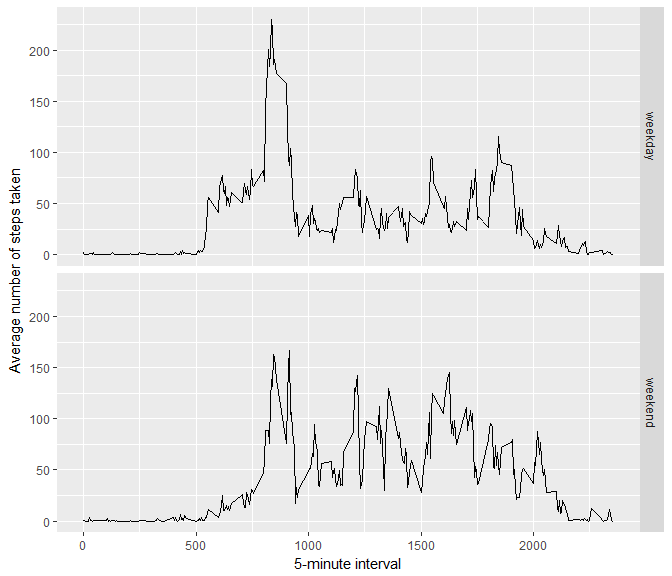
\includegraphics{PA1_template_files/figure-latex/Panel_Plot-1.pdf}


\end{document}
